\documentclass[12pt,a4paper,openany,twoside,cap]{ctexbook}
%-------------------------------------宏包引用---------------------------------------------------
\usepackage[paperwidth=185mm,paperheight=230mm,textheight=190mm,textwidth=145mm,left=20mm,right=20mm, top=25mm, bottom=15mm]{geometry}            %定义版面
%--------------------------------------------------------------------------------------
\usepackage{fontspec}
\usepackage{xunicode}
\usepackage{xltxtra}
%--------------------------------------------------------------------------------------
\usepackage[listings,theorems]{tcolorbox}
\usepackage{fancybox}                 % 边框,有阴影,fancybox提供了五种式样\fbox,\shadowbox,\doublebox,\ovalbox,\Ovalbox。
\usepackage{colortbl}                   % 单元格加背景
\usepackage{fancyhdr}                 % 页眉和页脚的相关定义
\usepackage[CJKbookmarks, colorlinks, bookmarksnumbered=true,pdfstartview=FitH,linkcolor=black]{hyperref}   % 书签功能,选项去掉链接红色方框
   %引用宏包所在位置
%-----------------------------------------------------主文档 格式定义---------------------------------
\addtolength{\headsep}{-0.1cm}        %页眉位置
%\addtolength{\footskip}{0.4cm}       %页脚位置
%-----------------------------------------------------设定字体等------------------------------
%\setmainfont{Times New Roman}    % 缺省字体
\setCJKfamilyfont{song}{SimSun}
\setCJKfamilyfont{hei}{FandolHei}
\setCJKfamilyfont{kai}{KaiTi}
\setCJKfamilyfont{fs}{FangSong}
\setCJKfamilyfont{li}{LiSu}
\setCJKfamilyfont{you}{YouYuan}
\setCJKfamilyfont{xingkai}{STXingkai}
\setCJKfamilyfont{xinwei}{STXinwei}
\setCJKfamilyfont{fzyao}{FZYaoTi}
\setCJKfamilyfont{fzshu}{FZShuTi}
%-------------------------------------------------------------------
\newCJKfontfamily\song{SimSun}
\newCJKfontfamily\hei{FandolHei}
\newCJKfontfamily\kai{FandolKai}
\newCJKfontfamily\fs{FangSong}
\newCJKfontfamily\li{LiSu}
\newCJKfontfamily\you{YouYuan}
\newCJKfontfamily\xingkai{STXingkai}
\newCJKfontfamily\xinwei{STXinwei}
\newCJKfontfamily\fzyao{FZYaoTi}
\newCJKfontfamily\fzshu{FZShuTi}
%-----------------------------------------------------------定义颜色---------------
\definecolor{blueblack}{cmyk}{0,0,0,0.35}%浅黑
\definecolor{darkblue}{cmyk}{1,0,0,0}%纯蓝
\definecolor{lightblue}{cmyk}{0.15,0,0,0}%浅蓝
%--------------------------------------------------------设定标题颜色--------------
\CTEXsetup[format+={\color{darkblue}}]{chapter}
\CTEXsetup[format+={\color{darkblue}}]{section}
\CTEXsetup[format+={\color{darkblue}}]{subsection}
%-----------------------------------------------------------定义、定理环境-------------------------
\newcounter{myDefinition}[chapter]\def\themyDefinition{\thechapter.\arabic{myDefinition}}
\newcounter{myTheorem}[chapter]\def\themyTheorem{\thechapter.\arabic{myTheorem}}
\newcounter{myCorollary}[chapter]\def\themyCorollary{\thechapter.\arabic{myCorollary}}

\tcbmaketheorem{defi}{定义}{fonttitle=\bfseries\upshape, fontupper=\slshape, arc=0mm, colback=lightblue,colframe=darkblue}{myDefinition}{Definition}
\tcbmaketheorem{theo}{定理}{fonttitle=\bfseries\upshape, fontupper=\slshape, arc=0mm, colback=lightblue,colframe=darkblue}{myTheorem}{Theorem}
\tcbmaketheorem{coro}{推论}{fonttitle=\bfseries\upshape, fontupper=\slshape, arc=0mm, colback=lightblue,colframe=darkblue}{myCorollary}{Corollary}
%------------------------------------------------------------------------------
\newtheorem{proof}{\indent\hei \textcolor{darkblue}{证明}}
\newtheorem{Solution}{\indent\hei \textcolor{darkblue}{解}}
%------------------------------------------------定义页眉下单隔线----------------
\newcommand{\makeheadrule}{\makebox[0pt][l]{\color{darkblue}\rule[.7\baselineskip]{\headwidth}{0.3pt}}\vskip-.8\baselineskip}
%-----------------------------------------------定义页眉下双隔线----------------
\makeatletter
\renewcommand{\headrule}{{\if@fancyplain\let\headrulewidth\plainheadrulewidth\fi\makeheadrule}}
\pagestyle{fancy}
\renewcommand{\chaptermark}[1]{\markboth{第\chaptername 章\quad #1}{}}    %去掉章标题中的数字
\renewcommand{\sectionmark}[1]{\markright{\thesection\quad #1}{}}    %去掉节标题中的点
\fancyhf{} %清空页眉
\fancyhead[RO]{\kai{\footnotesize.~\color{darkblue}\thepage~.}}         % 奇数页码显示左边
\fancyhead[LE]{\kai{\footnotesize.~\color{darkblue}\thepage~.}}         % 偶数页码显示右边
\fancyhead[CO]{\song\footnotesize\color{darkblue}\rightmark} % 奇数页码中间显示节标题
\fancyhead[CE]{\song\footnotesize\color{darkblue}\leftmark}  % 偶数页码中间显示章标题
%---------------------------------------------------------------------------------------------------------------------


    %格式所在位置
\begin{document}
\pagenumbering{Roman}    %Roman字体书写页码
%---------------------------------------------------封面等-----------------------

% ------------------------------封面--------------------------------------------
%\ctitle{数值计算方法\\{\vspace*{-1.2cm}\zihao{-2} SHUZHIJISUANFANGFA}}
%\cauthor{(第二版)\\吕同富~~康兆敏~~方秀男\hspace{1em}编著}
%\publisher{\centering
\includegraphics[totalheight=1.5in]{fig/qinghua.jpg}\\清华大学出版社$\cdot$北京}
%\makecover
% -----------------------------------------------------------------------------------
\title{\zihao{0}\hei\vspace*{-2cm} 数值计算方法\\{\vspace*{-1.2cm}\zihao{-2} SHUZHIJISUANFANGFA}}
\author{(第二版)\\吕同富~~康兆敏~~方秀男\hspace{1em}编著}
\date{\vspace*{3cm}\centering
\includegraphics[totalheight=1.5in]{fig/qinghua.jpg}\\清华大学出版社$\cdot$北京}
\maketitle
% -----------------------------------------------------------------------------------
                         %封面
\include{preface/intro}                          %简介
\markboth{序}{序} \vspace*{0.0cm}
\thispagestyle{empty}
\vspace*{2.2cm}
\centerline{\zihao{2}\hei{\color{darkblue}{第二版序}}}\vspace{2cm}

吕同富教授编著的《数值计算方法》
………………………………………………


\vspace{2cm}

\hfill XXXXXX\hspace{0.2em}

\hfill 2012年08月于XXXXXX\hspace{0.2em}
                        %序
\markboth{第二版前言}{第二版前言} \vspace*{0.0cm}
\thispagestyle{empty}
\vspace*{2.2cm}
\centerline{\zihao{2}\hei{\color{darkblue}{第二版前言}}}\vspace{2cm}

从2008年《数值计算方法》出版以来,得到了很多老师的关注,收到了很多读者的Email,给了很多的肯定和鼓励,同时也对书中的内容、体系、讲法等方面提出了很多宝贵的修改意见,借此再版之机,
向关心和支持作者工作的广大读者朋友表示深切谢意.此次再版,根据广大读者的建议,对原《数值计算方法》的内容作了适当的增删,在保持原《数值计算方法》特色的前提下,
对体例、格式、叙述、内容等方面作了较大的修改,力求使原《数值计算方法》的优点得到发展,缺点得到克服.其中很多章节和例题都重写了,修改后的内容更符合现代《数值计算方法》教学改革实际,
即便于教学,又有利于培养学生解决实际问题的能力.此次再版包括:非线性方程的数值解法;线性方程组的数值解法;矩阵特征值与特征向量的数值算法;插值方法;函数逼近;数值积分;数值微分;
常微分方程数值解等内容.由于课时体系等原因,删除了一些过时的内容,还有对部分过难的例题和习题作了修改和替换,新增了数字教学资源电子教案(PPT版由方秀男制作,PDF版吕同富制作),
MATLAB实验等内容供师生参考(相关数字教学资源可到清华大学出版社网上下载,也可以给作者发Email索取).本次再版由吕同富教授执笔.另外还有康兆敏副教授,
方秀男副教授编写了部分内容及习题和答案.全书由吕同富教授统稿.清华大学出版社佟丽霞编辑,几年来自始至终给作者以支持和鼓励,还有XXXXXX编辑用高度的责任感认真地编辑审校了书稿,
纠正了原稿中的很多不妥和疏漏,这里向他们及本书所列参考文献的作者们,以及为本书再版给予热心支持和帮助的朋友们,表示衷心的感谢.

本书可作为理工科本科生研究生数值计算方法课程教材或参考书,也可作为科技人员使用数值计算方法和MATLAB的参考手册.


\vspace{1cm}

\hfill 吕同富\hspace{0.2em}

\hfill ltongfu@126.com \hspace{0.2em}

\hfill 2012年08月\hspace{0.2em}
                   %二版前言
\markboth{第一版前言}{第一版前言} \vspace*{0.0cm}
\thispagestyle{empty}
\vspace*{2.2cm}
\centerline{\zihao{2}\hei{\color{darkblue}{第一版前言}}}\vspace{2cm}

数值计算方法与计算机相结合是本书的特点,也是科学计算发展的需要.
随着计算机的不断发展和进步,优秀的数学软件MATLAB应运而生,
MATLAB一问世就以它强大的功能,被广大科技工作者公认为科学计算最好的软件之一.
为使数值分析与MATLAB更好地结合,我们以最新版MATLAB为平台,编写了新版
《数值计算方法》,这也是数值计算方法教材发展进步的必然结果.

本书介绍了数值计算方法.内容涉及数值计算方法的数学基础、
数值计算方法在工程、科学和数学问题中的应用以及MATLAB程序等,涵盖了经典
数值分析的全部内容:包括非线性方程的数值解法;线性方程组的数值解法;
矩阵特征值与特征向量的数值算法;插值方法;函数逼近;数值积分;数值微分;
常微分方程数值解等.重点讲述数值分析方法的思想和原理,尽可能避免过深的数学理论
和过于繁杂的算法细节.
基于MATLAB是本书的特色.数值计算方法与科学计算软件MATLAB相结合,
有助于读者更有效地利用MATLAB的超强功能,来处理科学计算问题,有助于避免那种学过
数值计算方法但不能上机解决实际问题的现象发生.

在编写过程中,参考了国内已出版的同类教材(参考文献[1]~[23]),吸收了他们的
许多精华和优点,在题材的选取上作了一些变动,适当地增加了一些新内容,对书中
所有的数值方法都给出了MATLAB程序,有大量详实的应用实例可供参考,
有相当数量的习题可供练习.

本书取材新颖、阐述严谨、内容丰富、重点突出、推导详尽、思路清晰、深入浅出、
富有启发性,便于教学与自学.

全书内容由吕同富教授主持编写.具体分工:方秀男编写第1章和第2章;康兆敏
编写第3章;吕同富编写第4章至第9章.吉林大学周蕴时教授,哈尔滨工业大学吴勃英教授,
认真地阅读了本书,纠正了书中很多错误,并提出了许多保贵的修改意见;吉林大学马富明教授审定了书稿.
这里向他们及本书所列参考文献的作者们,清华大学出版社的佟丽霞和王海燕,
以及为本书出版给予热心支持和帮助的朋友们,表示衷心地感谢.

本书可作为理工科本科生研究生数值计算方法课程教材或参考书,也可作为科技人员
使用数值计算方法和MATLAB的参考手册.

出好书,使千百万莘莘学子受益,一直是作者追求的目标.但由于水平所限,尽管作了很大
努力,可能还会有很多不妥甚至是错误,望广大读者给予批评指正,谢谢.



\vspace{2cm}

\hfill 吕同富\hspace{0.2em}

\hfill ltongfu@126.com \hspace{0.2em}

\hfill 2008年03月\hspace{0.2em}
                     %前言
%%\thispagestyle{empty} %ȡ����ǰҳ��
\chapter{ժ\quad Ҫ}
\markboth{��~��~ժ~Ҫ}{��~��~ժ~Ҫ}
\vspace{0.5cm}

ժҪ����

{\hei �ؼ��ʣ�}
             %中文摘要
%%\thispagestyle{empty} %ȡ����ǰҳ��
 \chapter*{Abstract}
 \markboth{Ӣ~��~ժ~Ҫ}{Ӣ~��~ժ~Ҫ}
 \addcontentsline{toc}{chapter}{Abstract}
 \vspace{0.5cm}

 discussed in the former chapters.

 {\bf Key Words: }{\bf word1}
             %英文摘要
%-------------------------------------目录部分------------------------------------------
\setcounter{page}{1}   %重新开始页码
\renewcommand\contentsname{目\qquad 录}
%-------------------下面善三行去掉了目录首页页码---------------------
\makeatletter
\let\ps@plain\ps@empty
\makeatother
%-------------------------------------------------------------------------
\tableofcontents                                    %目录
%\addtocontents{toc}{\protect\begin{multicols}{2}}       %目录分两栏开始
\mainmatter    %前言和目录页码结束,正文重新开始设置页码
%-----------------------------------------正文开始------------------------------
\chapter{序论}
\thispagestyle{empty}

\setlength{\fboxrule}{0pt}\setlength{\fboxsep}{0cm}
\noindent\shadowbox{
\begin{tcolorbox}[arc=0mm,colback=lightblue,colframe=darkblue,title=学习目标与要求]
\kai\textcolor{darkblue}{1.~~了解科学计算的一般过程.}\\
\kai\textcolor{darkblue}{2.~~了解数值计算方法的研究内容和特点.}\\
\kai\textcolor{darkblue}{3.~~理解数值计算误差的有关概念.}\\
\kai\textcolor{darkblue}{4.~~掌握数值计算误差的控制方法.}
\end{tcolorbox}}
\setlength{\fboxrule}{1pt}\setlength{\fboxsep}{4pt}


\section{Colored boxes}

\begin{tcolorbox}[colback=red!5,colframe=red!75!black]
  My box.
\end{tcolorbox}

\begin{tcolorbox}[colback=blue!5,colframe=blue!75!black,title=My title]
  My box with my title.
\end{tcolorbox}

\begin{tcolorbox}[colback=green!5,colframe=green!75!black]
  Upper part of my box.
  \tcblower
  Lower part of my box.
\end{tcolorbox}

\begin{tcolorbox}[colback=yellow!5,colframe=yellow!75!black,title=My title]
  I can do this also with a title.
  \tcblower
  Lower part of my box.
\end{tcolorbox}

\begin{tcolorbox}[colback=yellow!10,colframe=red!75!black,lowerbox=invisible,
  savelowerto=\jobname_ex.tex]
  Now, we play hide and seek. Where is the lower part?
  \tcblower
  I'm invisible until you find me.
\end{tcolorbox}

\begin{tcolorbox}[colback=yellow!10,colframe=red!75!black,title=Here I am]
  \input{\jobname_ex.tex}
\end{tcolorbox}


\begin{tcolorbox}[colback=blue!50,colframe=blue!25!black,coltext=yellow,
    fontupper=\Large\bfseries,arc=6mm,boxrule=2mm,boxsep=5mm]
  Funny settings.
\end{tcolorbox}

\subsection{\LaTeX-Table}

\begin{table}[h]\begin{center}\color{darkblue}\caption{计算结果}\color{black}\label{tab1-2}
{\footnotesize
\begin{tabular}{r|r||r|r||r|r||r|r}\arrayrulecolor{darkblue}\hline\rowcolor{lightblue}
  $n$&$I_n$&$n$&$I_n$&$n$&$I_n$&$n$&$I_n$\\\hline
  19&0.008\ 3&14&0.011\ 2&9&0.016\ 9&4&0.034\ 3\\
  18&0.008\ 9&13&0.012\ 0&8&0.018\ 8&3&0.043\ 1\\
  17&0.009\ 3&12&0.013\ 0&7&0.021\ 2&2&0.058\ 0\\
  16&0.009\ 9&11&0.014\ 1&6&0.024\ 3&1&0.088\ 4\\
  15&0.010\ 5&10&0.015\ 4&5&0.028\ 5&0&0.182\ 3\\\hline
 \end{tabular}}\end{center}\end{table}


\section{\LaTeX-Examples}

\begin{tcblisting}{colback=red!5,colframe=red!75!black}
This is a \LaTeX\ example:
$\displaystyle\sum\limits_{i=1}^n i = \frac{n(n+1)}{2}$.
\end{tcblisting}


\section{Theorems}

\begin{defi}{Summation of Numbers}{defi1.1}
  For all natural number $n$ it holds:\\[2mm]
  $\displaystyle\sum\limits_{i=1}^n i = \frac{n(n+1)}{2}$.
\end{defi}

\begin{theo}{Summation of Numbers}{theo1.1}
  For all natural number $n$ it holds:\\[2mm]
  $\displaystyle\sum\limits_{i=1}^n i = \frac{n(n+1)}{2}$.
\end{theo}

\begin{coro}{Summation of Numbers}{coro1.1}
  For all natural number $n$ it holds:\\[2mm]
  $\displaystyle\sum\limits_{i=1}^n i = \frac{n(n+1)}{2}$.
\end{coro}
We have given Theorem \ref{Theorem:theo1.1} on page \pageref{Theorem:theo1.1}.



\begin{table}[h]\begin{center}\color{darkblue}\caption{计算结果}\color{black}\label{tab1-1}
{\footnotesize
\begin{tabular}{r|r||r|r||r|r||r|r}\arrayrulecolor{darkblue}\hline\rowcolor{lightblue}
  $n$&$I_n$&$n$&$I_n$&$n$&$I_n$&$n$&$I_n$\\\hline
  1&0.088\ 4&6&0.034\ 4&11&-31.392\ 5&16&9.814\ 5e+4\\
  2&0.581\ 0&7&-0.029\ 0&12&157.045\ 7&17&-4.907\ 3e+5\\
  3&0.043\ 1&8&0.270\ 1&13&-785.151\ 6&18&2.453\ 6e+6\\
  4&0.347\ 0&9&-1.239\ 3&14&3.925\ 8e+3&19&-1.226\ 8e+7\\
  5&0.026\ 5&10&0.296\ 7&15&-1.962\ 9e+4&20&6.134\ 1e+7\\\hline
\end{tabular}}\end{center}\end{table}

\section{graphicx}

\begin{figure}[h]
\begin{minipage}[t]{0.5\linewidth}
\centering
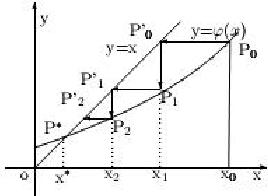
\includegraphics[totalheight=1.2in]{fig/tu2-2}
\caption{不动点迭代法收敛} \label{fig:tu2-2}
\end{minipage}
\begin{minipage}[t]{0.5\linewidth}
\centering
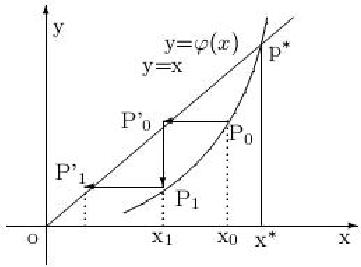
\includegraphics[totalheight=1.3in]{fig/tu2-3}
\caption{不动点迭代法发散} \label{fig:tu2-3}
\end{minipage}
\end{figure}



\vspace{0.5cm}
\addcontentsline{toc}{section}{\protect\numberline{}{习题一}}
\markboth{习题一}{习题一} \centerline{\textcolor{darkblue}{\hei\zihao{4}
 习题一}}\vspace{0.5cm}


       %第一章
%\include{book/chap2}       %第二章
%\include{book/chap3}       %第三章
%\include{book/chap4}       %第四章
%\include{book/chap5}       %第五章
%\include{book/chap6}       %第六章
%\include{book/chap7}       %第七章
%\include{book/chap8}       %第八章
%\include{book/chap9}       %第九章
%\addtocounter{chapter}{7}
%-----------------------------------------正文结束------------------------------
\markboth{部分习题答案}{部分习题答案}
%\clearpage  %清楚前面的偶数空白页
\phantomsection %加这个命令后,目录中的超链接才指向正确的页码
\addcontentsline{toc}{chapter}{\protect\numberline{}{\hspace{-1.5em}部分习题答案}}
\thispagestyle{empty}
\vspace*{2.2cm}
\centerline{\zihao{2}\hei{\color{darkblue}{部分习题答案}}}

\vspace{2cm}\centerline{\textcolor{darkblue}{\hei\zihao{4} 习题一}}\vspace{0.5cm}


1.有7位有效数字

2.~~816.96,\qquad 6.0000,\qquad 17.323,\qquad 1.2357,\qquad 93.182,\qquad 0.015236.

3.~~5位,3位,6位,4位.

4.~~2位有效数字.

5.~~0.020685.

6.~~3位,3位.

7.~~$0.5\times10^{-4}$,~~~~~~$0.8\times10^{-2}$.


      %习题答案
%\addtocontents{toc}{\protect\end{multicols}}   %目录分两栏结束
\begin{thebibliography}{99}
\addcontentsline{toc}{chapter}{\protect\numberline{}{\hspace{-1.5em}参考文献}}
\markboth{参考文献}{参考文献}
\bibitem{a}魏毅强,张建国,张洪斌等.数值计算方法.北京:科学出版社,2004,8
\bibitem{b}黄铎,陈兰平,王风.数值分析.北京:科学出版社,2004,3
\bibitem{c}华中理工大学数学系.计算方法.北京:高等教育出版社,1999,9
\bibitem{d}姜健飞,胡良剑,唐俭.数值分析及其MATLAB实验.北京:科学出版社,2004,6
\bibitem{e}薛毅.数值分析与实验.北京:北京工业大学出版社,2005,3
\bibitem{f}张可村,赵英良.数值计算的算法与分析.北京:科学出版社,2004,6
\bibitem{g}石瑞民,许志刚,孙靖.数值计算.北京:高等教育出版社,2004,6
\bibitem{h}黄明游,刘播,徐涛.数值计算方法.北京:科学出版社,2005,8
\bibitem{i}李庆杨,王能超,易大义.数值分析.北京:清华大学出版社,2001,8
\bibitem{j}沈剑华.数值计算基础.上海:同济大学出版社,1999,5
\bibitem{k}李庆扬,关治,白峰山.数值计算原理.北京:清华大学出版社,2000,9
\bibitem{l}吴勃英,王德明,丁效华,李道华.数值分析原理.北京:科学出版社,2004,2
\bibitem{m}林成森.数值计算方法.北京:科学出版社,2005,1
\bibitem{n}蔺小林,蒋耀林.现代数值分析.北京:国防工业出版社,2004,9
\bibitem{o}崔国华.计算方法.武汉:华中理工大学出版社,2001,3
\bibitem{p}合肥工业大学数学与信息科学系.数值计算方法.合肥:合肥工业大学出版社,2004,3
\bibitem{q}张铮,杨文平,石博强等.MATLAB程序设计与实际应用.北京:中国铁道出版社,2003,11
\bibitem{r}张志涌等.精通MATLAB.北京:北京航空航天大学出版社,2003,8
\bibitem{s}清源计算机工作室.MATLAB高级应用.北京:机械工业出版社,2000,6
\bibitem{t}马富明等.数值分析(上).北京:高等教育出版社,2007,5
\bibitem{u}马富明等.数值分析(下).北京:高等教育出版社,2008,2
\bibitem{v}张平文,陈铁军.数值分析.北京:北京大学出版社,2007,1
\bibitem{w}易大义,陈道琦.数值分析引论.杭州:浙江大学出版社,1998,9
\end{thebibliography}
                               %参考文献部分
\clearpage
\end{document}

